%%% Exemplo de utilização da classe ITA
%%%
%%%   por        Fábio Fagundes Silveira   -  ffs [at] ita [dot] br
%%%              Benedito C. O. Maciel     -  bcmaciel [at] ita [dot] br
%%%              Giovani Volnei Meinertz   -  giovani [at] ita [dot] br
%%%    	         Hudson Alberto Bode       -  bode [at] ita [dot]br
%%%    	         P. I. Braga de Queiroz    -  pi [at] ita [dot] br
%%%    	         Jorge A. B. Gripp         -  gripp [at] ita [dot] br
%%%    	         Juliano Monte-Mor         -  jamontemor [at] yahoo [dot] com [dot] br
%%%    	         Tarcisio A. B. Gripp      -  tarcisio.gripp [at] gmail [dot] com
%%%
%%%   Versão para overleaf:
%%%   por        Alejandro A. Rios Cruz    - aarc.88@gmail.com
%%%              Saulo Gómez               - sagomezs@unal.edu.co
%%%              Ocimar Santos             - ocimar.acad@gmail.com
%%%
%%%   Template disponibilizado em:
%%%              Overleaf: https://pt.overleaf.com/latex/templates/thesis-template-aeronautics-institute-of-technology-ita/yhfrqqydpygk
%%%
%%%   Contribuia você também!
%%%              GitHub:   https://github.com/gabriellnuness/Template_Thesis_ITA
%%%
%%%  IMPORTANTE: O texto contido neste exemplo nao significa absolutamente nada.  :-)
%%%              O intuito aqui eh demonstrar os comandos criados na classe e suas
%%%              respectivas utilizacoes.
%%%
%%%  Tese.tex  2016-08-25
%%%  $HeadURL: http://www.apgita.org.br/apgita/teses-e-latex.php $
%%%
%%% ITALUS
%%% Instituto Tecnológico de Aeronáutica --- ITA, Sao Jose dos Campos, Brasil
%%%                   http://groups.yahoo.com/group/italus/
%%% Discussion list: italus {at} yahoogroups.com
%%%
%++++++++++++++++++++++++++++++++++++++++++++++++++++++++++++++++++++++++++++++
% Para alterar o TIPO DE DOCUMENTO, preencher a linha abaixo \documentclass[?]{?}
%   \documentclass[tg]{ita}			= Trabalho de Graduacao
%   \documentclass[tgfem]{ita}	= Para Engenheiras
%   								msc     		= Dissertacao de Mestrado
%   								mscfem   		= Para Mestras
%   								dsc      		= Tese de Doutorado
%   								dscfem   		= Para Doutoras
%   								quali    		= Exame de Qualificacao
%   								qualifem 		= Exame de Qualificacao para Doutoras
% Para 'Draft Version'/'Versao Preliminar' com data no rodape, adicionar 'dv':
%   \documentclass[dsc, dv]{ita}
% Para trabalhos em Inglês, adicionar 'eng':
%   \documentclass[dsc, eng]{ita}
%		\documentclass[dsc, eng, dv]{ita}
%++++++++++++++++++++++++++++++++++++++++++++++++++++++++++++++++++++++++++++++
\documentclass[msc,eng]{ita}    % ITA.cls based on standard book.cls
% Quando alterar a classe, por exemplo de [msc] para [msc, eng]) rode mais uma vez o botão BUILD OUTPUT caso haja erro
\usepackage{ae}
\usepackage{graphicx}


\usepackage{epsfig}
\usepackage{amsmath}
\usepackage{amssymb}
\usepackage{subfig}
\usepackage{multirow}
\usepackage{float}
\usepackage{amsthm}
\usepackage{url}         % formats URL addresses properly
\usepackage{appendix}    % allows appendix section to be included
\usepackage{lscape}      % allows a page to be rendered in landscape mode
\usepackage{multicol}    % allows text in multi columns
\usepackage{cancel}      % needed to show canceled terms in equations
\usepackage{lettrine}
\usepackage{float}
\usepackage{placeins}

% Bibliography resource (biblatex is already configured in ita.cls)
\addbibresource{Referencias/referencias.bib}

% --- Add this to your PREAMBLE (before \begin{document}) ---

\usepackage{listings} % For code listings
\usepackage{xcolor}   % For custom colors
\usepackage{inconsolata} % A nice monospaced font for code

% Define custom colors for the code style
\definecolor{codegreen}{rgb}{0,0.6,0}
\definecolor{codegray}{rgb}{0.5,0.5,0.5}
\definecolor{codepurple}{rgb}{0.58,0,0.82}
\definecolor{backcolour}{rgb}{0.95,0.95,0.95}

% Define the code style using lstset
\lstdefinestyle{mystyle}{
    backgroundcolor=\color{backcolour},   
    commentstyle=\color{codegreen},
    keywordstyle=\color{magenta},
    numberstyle=\tiny\color{codegray},
    stringstyle=\color{codepurple},
    basicstyle=\ttfamily\small, % Use inconsolata font if installed
    breakatwhitespace=false,         
    breaklines=true,                 
    captionpos=b,                    
    keepspaces=true,                 
    numbers=left,                    
    numbersep=5pt,                  
    showspaces=false,                
    showstringspaces=false,
    showtabs=false,                  
    tabsize=2,
    frame=single, % Adds a frame around the code
    rulecolor=\color{black!30}, % Light gray color for the frame
}

% Apply this style to all subsequent listings
\lstset{style=mystyle}


%HHHHHHHHHHHHHHHHHHHHHHHHHHHHHHHHHHHHHHHHHHHHHHHHHHHHHHHHHHHHHHHHHHHHHHHHHHHHHHHHHHHHHHHHHHHHHHHHHHHHHHHHHHHH
% Bibliography resource already defined above
%HHHHHHHHHHHHHHHHHHHHHHHHHHHHHHHHHHHHHHHHHHHHHHHHHHHHHHHHHHHHHHHHHHHHHHHHHHHHHHHHHHHHHHHHHHHHHHHHHHHHHHHHHHHH
%\usepackage{subfigure}
%\usepackage{subfigmat}
%PACOTEFIGURAS_SE _ERRADO_ESXCLUIR_ACIMA
\usepackage{booktabs}
%PACOTETABELAS_SE _ERRADO_ESXCLUIR_ACIMA
%HHHHHHHHHHHHHHHHHHHHHHHHHHHHHHHHHHHHHHHHHHHHHHHHHHHHHHHHHHHHHHHHHHHHHHHHHHHHHHHHHHHHHHHHHHHHHHHHHHHHHHHHHHHH

%++++++++++++++++++++++++++++++++++++++++++++++++++++++++++++++++++++++++++++++
% Espaçamento padrão de todo o documento
%++++++++++++++++++++++++++++++++++++++++++++++++++++++++++++++++++++++++++++++
\onehalfspacing

%singlespacing Para um espaçamento simples
%onehalfspacing Para um espaçamento de 1,5
%doublespacing Para um espaçamento duplo

%++++++++++++++++++++++++++++++++++++++++++++++++++++++++++++++++++++++++++++++
% Identificacoes (se o trabalho for em inglês, insira os dados em inglês)
% Para entradas abreviadas de Professora (Profa.) em português escreva: Prof$^\textnormal{a}$.
%++++++++++++++++++++++++++++++++++++++++++++++++++++++++++++++++++++++++++++++
\course{Engenharia da Computação}  % Programa de PG ou Curso de Graduação
%\area{Aircraft Design} % Área de concentração na PG (Não utilizado no caso de TG)

% Autor do trabalho: Nome Sobrenome
\authorgender{masc}                     %sexo: masc ou fem
\author{Fernando}{Gusmão Zanchitta}
\itaauthoraddress{Av. Jorge Zarur 231, Bl 6, Ap.301}{12.243-081}{São José dos Campos--SP}

% Titulo da Tese/Dissertação
\title{Large Language Models for Automated Program Repair: An Empirical Study with Tracebacks and Prompt Engineering}

% Orientador
\advisorgender{masc}                    % masc ou fem
\advisor{Prof.~Dr.}{Filipe Alves Neto Verri}{ITA}

% Coorientador (Caso não haja coorientador, colocar ambas as variáveis \coadvisorgender e \coadvisor comentadas, com um % na frente)
% \coadvisorgender{fem}									% masc ou fem
% \coadvisor{Prof$^\textnormal{a}$.~Dr$^\textnormal{a}$.}{Doralice Serra}{OVNI}

% Pró-reitor da Pós-graduação
\bossgender{masc}												% masc ou fem
\boss{Prof.~Dr.}{... INSERIR}

% %Coordenador do curso no caso de TG
% \bosscoursegender{masc}									% masc ou fem
% \bosscourse{Prof.~Dr.}{John Walker}

% Palavras-Chaves informadas pela Biblioteca -> utilizada na CIP
\kwcip{Automatic Program Repair}
\kwcip{Large Language Model}
\kwcip{Prompt Engineering}


% membros da banca examinadora

\examiner{Prof. Dr.}{Alan Turing}{Presidente}{ITA}
\examiner{Prof. Dr.}{Linus Torwald}{}{UXXX}
\examiner{Prof. Dr.}{Richard Stallman}{}{UYYY}
\examiner{Prof. Dr.}{Donald Duck}{}{DYSNEY}
\examiner{Prof. Dr.}{Mickey Mouse}{}{DISNEY}

% Data da defesa (mês em maiúsculo, se trabalho em inglês, e minúsculo se trabalho em português)
\date{23}{novembro}{2025}

% Número CDU - (somente para TG)
% \cdu{???.??}

% Glossario
\makenoidxglossaries % to use glossaries pkg
\frontmatter


%%%%%%%% acronyms %%%%%%%%
\newacronym{ctq}{CTq}{computed torque}
\newacronym{dc}{DC}{direct current}
\newacronym{ear}{EAR}{Equação Algébrica de Riccati}
\newacronym{graus_liberdade}{GDL}{graus de liberdade}
\newacronym{isr}{ISR}{interrupção de serviço e rotina}
\newacronym{lasi}{LASI}{Laboratório	de sistemas inteligentes}


\newglossaryentry{comprimento}{name=\ensuremath{\alpha}, description={Comprimento}, sort={a}}

\newglossaryentry{altura}{name=\ensuremath{\beta}, description={Altura}, sort={b}}

\newglossaryentry{velocidade}{name=\ensuremath{v}, description={Velocidade}, sort={v}}

\newglossaryentry{vet_distancia}{name=\ensuremath{\textbf{a}}, description={Vetor de distâncias}, sort={a_bold}}

\newglossaryentry{vet_unitario}{name=\ensuremath{\textbf{e}_{j}}, description={Vetor unitário de dimensão $n$ e com o $j$-ésimo componente igual a $1$}, sort={e_j}}

\newglossaryentry{delta_kro}{name=\ensuremath{\delta_{k-k_f}}, description={Delta de Kronecker no instante $k_f$}, sort={d_k}}



\begin{document}
% Folha de Rosto e Capa para o caso do TG
\maketitle

% Dedicatoria: Nao esqueca essa secao  ... :-)
\begin{itadedication}
Aos amigos da Graduação e Pós-Graduação do ITA por motivarem tanto a criação deste template pelo Fábio Fagundes Silveira quanto por motivarem a mim e outras pessoas a atualizarem e aprimorarem este excelente trabalho.
\end{itadedication}

% Agradecimentos
\begin{itathanks}
Primeiramente, gostaria de agradecer ao Dr. Donald E. Knuth, por ter desenvolvido o \TeX.

Ao Dr. Leslie Lamport, por ter criado o \LaTeX, facilitando muito a utilização do \TeX, e assim, eu não ter que usar o Word.

Ao Prof. Dr. Meu Orientador, pela orientação e confiança depositada na realização deste trabalho.

Ao Dr. Nelson D'Ávilla, por emprestar seu nome a essa importante via de trânsito na cidade de São José dos Campos.

Ah, já estava esquecendo... agradeço também, mais uma vez ao \TeX, por ele não possuir vírus de macro :-)

\end{itathanks}

% Epígrafe
\thispagestyle{empty}
\ifhyperref\pdfbookmark[0]{\nameepigraphe}{epigrafe}\fi
\begin{flushright}
\begin{spacing}{1}
\mbox{}\vfill
{\sffamily\itshape
``If I have seen farther than others,\\
it is because I stood on the shoulders of giants.''\\}
--- \textsc{Sir~Isaac Newton}

\end{spacing}
\end{flushright}

% Resumo
\begin{abstract}
\noindent
Placeholder abstract
\end{abstract}

% Abstract
\begin{englishabstract}
\noindent
Well, the book is on the table. This work presents a control methodologie for the position of the  passive joints of an underactuated manipulator in a suboptimal way. The term underactuated refers to the fact that not all the joints or degrees of freedom of the system are equipped with actuators, which occurs in practice due to failures or as design result. The passive joints of manipulators like this are indirectly controlled by the motion of the active joints using the dynamic coupling characteristics. The utilization of actuation redundancy of the active joints allows the minimization of some criteria, like energy consumption, for example. Although the kinematic structure of an underactuated manipulator is identical to that of a similar fully actuated one, in general their dynamic characteristics are different due to the presence of passive joints. Thus, we present the dynamic modelling of an underactuated manipulator and the concept of coulpling index. This index is used in the sequence of the optimal control of the manipulator.

\end{englishabstract}

% Lista de figuras
\listoffigures %opcional

% Lista de tabelas
\listoftables %opcional

% Lista de abreviaturas
\printnoidxglossary[type=\acronymtype,
    title=\listofabbreviationsname,
    toctitle=\listofabbreviationsname,
    sort=standard,
    nonumberlist]
    
% Lista de simbolos
\printnoidxglossary[
    title=\listofsymbolsname,
    toctitle=\listofsymbolsname,
    sort=standard,
    nonumberlist]

% Sumario
\tableofcontents


\mainmatter
% Os capitulos comecam aqui

\chapter{Introduction and Background}
This chapter covers the motivation for this thesis, along with research goals, research
questions, and a list of contributions.

\section{Motivation}
%todo Brief overview of APR
Modern software systems continuously evolve with inevitable bugs due to feature deprecation, new features added, and refactoring. These bugs are widely known as a destructive problem, generating costs up to trillions of dollars every year.%todo: \cite{todo}.

Bugs and errors in code are a recurring problem in the software industry, leading to collateral effects of multiple sizes. %\cite{todo} 
As a consequence, there is a substantial amount of time spent only to solve these problems in an efficient way with litle or no human intervention.

In APR research of the last decade, most of traditional methods include search-based, constraint-based, and template-based approaches.%todo cite
These studies led to the development of methods such of SimFix, VarFix, SearchRepair, and Tfix.
More recent studies use machine learning and deep learning techniques were employed to improve program repair tasks.
% cite
With the growth of Large Language Models (LLMs), the Software Engineering area was significantly transformed, specially due to Code LLMs. These models are either pretrained or finetuned on programming languages, directly affecting areas such as code summarization, code generation, bug detection and also APR.


%todo Challenges in traditional methods

%todo Introduction to LLMs as potential solution



\section{Problem Statement}
%todo Description of the problem, and limitations of traditional methods

%todo Description of the problem, and limitations of LLMs. Gap between sytactical and semantic correctness.

\section{Objective and Research Questions} 
 %todo Change to Objective and Research Questions
%todo Objective of the thesis
Esse projeto busca estudar diferentes técnicas de prompt engineering, em realizar tarefas de Patch Correction dentro do campo de Automated Program Repair (APR).


\textbf{RQ1: Comparison between specialized code models vs general-purpose models?}

\textbf{RQ2: Does style based prompt improve the overall effectiveness of responses?}

\textbf{RQ3: Does system prompt improve performances of APR tasks?}


\section{Contribution}

\chapter{Related Works}
\section{Experiment Setup}
\subsection{Motivation}

During Automated Program Repair (APR) activities, traditional methods (based on heuristics or templates) often generate syntactically correct changes, but they fall short in the semantic and code style aspects (insert ref).

In this context, Large Language Models (LLMs) are capable of capturing code patterns and semantic context with high precision.
On the other hand, LLMs exhibit significant sensitivity to how their instructions (prompts) are phrased. Different instructions can alter the fidelity to the original style, the clarity of the patch, and the size of the modification, especially if little context is provided during the correction process (insert ref).

\subsection{Dataset}

The experiment uses the Pytracebugs dataset \cite{Pytracebugs}, which contains Python source codes from GitHub repositories at the granularity of function snippets and their corresponding Traceback errors; see the example below.


\begin{figure}[h!]
    \centering
    \caption{An example of a single data point from the Pytracebugs dataset.}
    \label{fig:dataset-example}

    % (a) The Buggy Code
    \begin{lstlisting}[
        language=Python,
        frame=single,
        basicstyle=\ttfamily\small,
        caption={a) Buggy Code Snippet (\texttt{before\_merge})},
        belowcaptionskip=-0.5em % Adjust spacing
        ]
def noise(self, value):
  self.noise_covar.initialize(value)
    \end{lstlisting}

    % (b) The Traceback Error
    \begin{lstlisting}[
        frame=single,
        basicstyle=\ttfamily\small,
        caption={b) Traceback Error (\texttt{full\_traceback})},
        belowcaptionskip=-0.5em % Adjust spacing
        ]
import gpytorch
gl = gpytorch.likelihoods.GaussianLikelihood()
gl.initialize(noise=1)
Traceback (most recent call last):
File ""<stdin>"", line 1, in <module>
File "".../gpytorch/gpytorch/module.py"", line 89, in initialize
setattr(self, name, val)
File ""../lib/python3.6/site-packages/torch/nn/modules/module.py"", line 579, in __setattr__
object.__setattr__(self, name, value)
File "".../gpytorch/gpytorch/likelihoods/gaussian_likelihood.py"", line 63, in noise
self.noise_covar.initialize(value)
TypeError: initialize() takes 1 positional argument but 2 were given
    \end{lstlisting}

    % (c) The Fixed Code
    \begin{lstlisting}[
        language=Python,
        frame=single,
        basicstyle=\ttfamily\small,
        caption={c) Fixed Code Snippet (\texttt{after\_merge})}
        ]
def noise(self, value):
  self.noise_covar.initialize(noise=value)
    \end{lstlisting}
\end{figure}

\begin{figure}[h!]
    \centering
    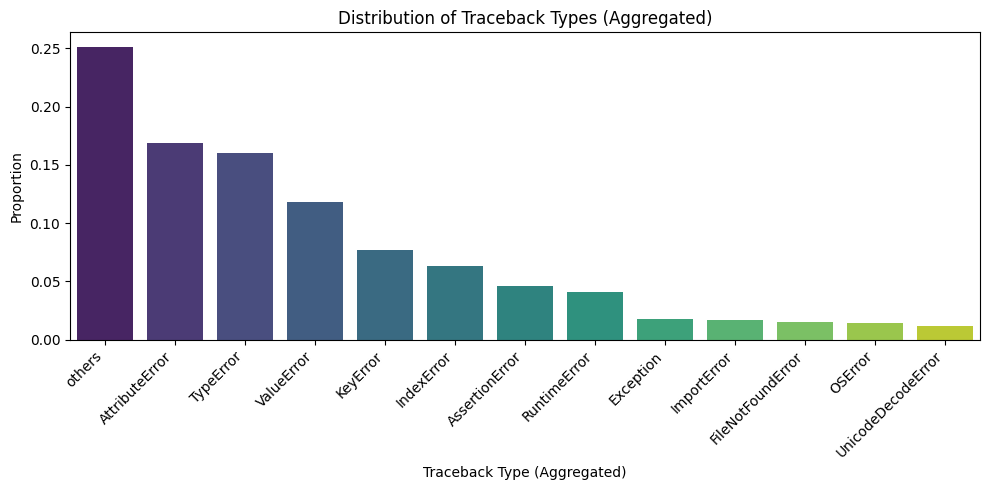
\includegraphics[width=0.7\textwidth]{Cap2/dataset-traceback-type.png}
    \caption{Distribution of Error Types in the dataset - Less than 1\% relevant are consolidated into 'others' category.}
    \label{fig:dataset-traceback-types}
\end{figure}

Most frequent traceback errors can be found in Figure \ref{fig:dataset-traceback-types}, with the most frequent ones being Atribute Error and TypeError with $16.84\%$ and $16\%$ of the values respectivelly. Also, there is a significant amount of erros that appear less than $1\%$ of the time, and were aggregated into the 'Others' Category.

%TODO: Adicionar exemplos de trabalhos publicados que utilizam como referencia o dataset proposto.
Some published works that use this dataset aim to study problems such as Vulnerability Detection \cite{zhao2024coding} and fault localization \cite{kulkarni2024graph}.

\subsection{LLM Models}
For the first experiment, four models were chosen. Two of these are open-source models specialized in code generation, considered state-of-the-art in this category: Qwen 2.5 coder 32b (instruct) \cite{hui2024qwen25codertechnicalreport} and Codestral 2501 \cite{Codestral_202501}. Additionally, two state-of-the-art, commonly used closed-source models of a relatively similar size were selected: Claude $3.5$ Sonnet and GPT $4o$ Model.

Although these models are all similarly competitive in structured benchmarks, they differ considerably in terms of usage cost. For reference, the token cost for each selected model is shown in Table \ref{tab:model-tokens}.
\begin{table}[h!]
\centering
\caption{Token usage price per model.}
\label{tab:model-tokens}
\begin{tabular}{|l|c|c|}
\hline
\textbf{Model} & \textbf{Input Tokens (1M)} & \textbf{Output Tokens (1M)} \\ \hline
Claude Sonnet 3.5 & \$3.0 & \$15.0 \\ \hline
Gpt 4o & \$2.5 & \$10 \\ \hline
Codestral 2501 & \$0.3 & \$0.9 \\ \hline
Qwen 2.5 Coder 32B Instruct & \$0.05 & \$0.20 \\ \hline
\end{tabular}
\end{table}
% todo addicionar gemini flas
%TODO melhorar a argumentação desses modelos
% Falar do tamanho dos modelos e da comparabilidade deles. Exibir ranking. Existem muitos, portanto qualquer escolha tem uma arbitrariedade. Não vamos todos no hugging faces.

% TODO trazer artigos que divulgam esses modelos.


\subsection{Prompts updated}

To test the model's sensitivity to the prompt's instructions, all prompts were formatted 
using a consistent template, shown in Listing \ref{lst:prompt-template}. This structure ensures 
that each model receives the context—buggy code and traceback error—in a clear, delimited 
format, and is explicitly asked to return only the corrected code.

% The 'figure' environment helps manage the placement and captioning of the listing.
\begin{figure}[h!]
% This is the crucial line that starts the code block.
% The formatting options are placed in the square brackets.
\begin{lstlisting}[
    caption={The general template used for all prompts.},
    label={lst:prompt-template},
    basicstyle=\ttfamily\small,
    frame=single,
    breaklines=true
]
{{ instruction_prompt }}

### BUGGY CODE:
{{ buggy_code }}

### ERROR:
{{ traceback_error }}

### RETURN ONLY THE CORRECTED CODE BELOW:

IMPORTANT: Return ONLY the corrected/requested code. Do not include any explanations, comments about the changes, or other text. Just return the pure code.

\end{lstlisting} % This line correctly ends the code block.
\end{figure}
% It clearly isolates the variable you are testing.
\begin{table}[h!]
\centering
\caption{Instruction variations for the \texttt{instruction\_prompt} variable.}
\label{tab:prompt-instructions}
\begin{tabular}{|l|p{0.55\textwidth}|p{0.15\textwidth}|}
\hline
\textbf{Prompt ID} & \textbf{Instruction Text} & \textbf{System Prompt} \\ \hline
P1 (Baseline) & You are a helpful assistant that corrects the code based on the traceback error. & False. \\\hline
P2 (Style-aware) & You are a helpful assistant that corrects the code based on the traceback error. You must respect the original code structure and the original code style. & False. \\ \hline
P3 (System Prompt) & You are a helpful assistant that corrects the code based on the traceback error. & True. \\ \hline
\end{tabular}
\end{table}
The core of the experiment lies in the variation of the \texttt{instruction\_prompt} placeholder and the addition of system prompt. 
We designed three distinct instructions, which we will refer to as P1 (Baseline) and P2 (Style-aware) and P3 (System Prompt), 
to evaluate the impact of a more detailed directive. The specific text for each instruction 
is detailed in Table \ref{tab:prompt-instructions}.

\subsection{Experiment tracking}
For each of the 4 models, 300 responses were executed for each of the prompts, totaling 4 x 300 x 3 = 3600 responses. For each response, the following metrics were evaluated: AST, AST-Normalized, CodeBLEU, N-gram match, Weighted N-gram match, Dataflow Match.
Each metric was compared against both the original (buggy) code and the ground truth correction.


\subsection{Implementation Details}
\label{sec:implementation-details}

All API calls to the proprietary models (GPT-4o and Claude 3.5 Sonnet) and the open-source models (Qwen 2.5 and Codestral) were managed through the \textbf{OpenRouter} API aggregation service. This approach was chosen to ensure a consistent and reproducible experimental setup across all models from a single interface.

The specific model identifiers used on the platform are listed below. To ensure that the results were as deterministic as possible and to facilitate a fair comparison, the generation parameters were kept constant for all API calls: a \textbf{temperature of 0} and a \textbf{top\_p of 1.0} were used. All experiments were conducted in \textbf{July 2025}.

\begin{itemize}
    \item \texttt{openai/gpt-4o}
    \item \texttt{anthropic/claude-3.5-sonnet}
    \item \texttt{qwen/qwen-2.5-coder-32b-instruct} 
    \item \texttt{mistralai/codestral-2501}
\end{itemize}

\subsubsection{Experimental Results Summary}
Table \ref{tab:comprehensive-results} presents the comprehensive results of our experiment, showing the performance of all four models across the three prompt conditions for each evaluation metric. The results are formatted as mean ± standard deviation to provide both central tendency and variability measures.

\begin{table}[h!]
\centering
\caption{Comprehensive metrics comparison across all models and prompt conditions (mean ± std).}
\label{tab:comprehensive-results}
\resizebox{\textwidth}{!}{%
\begin{tabular}{|l|l|c|c|c|c|c|c|c|c|}
\hline
\textbf{Model} & \textbf{Prompt} & \textbf{AST Score} & \textbf{Text Score} & \textbf{AST Norm.} & \textbf{CodeBLEU} & \textbf{N-gram} & \textbf{W. N-gram} & \textbf{Syntax} & \textbf{Dataflow} \\
\hline
\multirow{3}{*}{Claude 3.5 Sonnet} & Baseline & $0.22 \pm 0.36$ & $0.68 \pm 0.23$ & $0.29 \pm 0.40$ & $0.73 \pm 0.17$ & $0.64 \pm 0.27$ & $0.71 \pm 0.24$ & $0.76 \pm 0.19$ & $0.71 \pm 0.26$ \\
\cline{2-10}
& Style-aware & $0.23 \pm 0.37$ & $0.69 \pm 0.23$ & $0.31 \pm 0.41$ & $0.73 \pm 0.17$ & $0.64 \pm 0.26$ & $0.72 \pm 0.24$ & $0.77 \pm 0.19$ & $0.71 \pm 0.26$ \\
\cline{2-10}
& System & $0.23 \pm 0.36$ & $0.71 \pm 0.22$ & $0.38 \pm 0.44$ & $0.73 \pm 0.17$ & $0.65 \pm 0.26$ & $0.71 \pm 0.24$ & $0.76 \pm 0.19$ & $0.72 \pm 0.26$ \\
\hline
\multirow{3}{*}{Codestral 2501} & Baseline & $0.28 \pm 0.41$ & $0.75 \pm 0.21$ & $0.28 \pm 0.41$ & $0.78 \pm 0.19$ & $0.73 \pm 0.26$ & $0.77 \pm 0.24$ & $0.81 \pm 0.19$ & $0.74 \pm 0.26$ \\
\cline{2-10}
& Style-aware & $0.28 \pm 0.41$ & $0.75 \pm 0.22$ & $0.28 \pm 0.41$ & $0.78 \pm 0.18$ & $0.73 \pm 0.26$ & $0.77 \pm 0.24$ & $0.81 \pm 0.19$ & $0.75 \pm 0.26$ \\
\cline{2-10}
& System & $0.28 \pm 0.41$ & $0.75 \pm 0.21$ & $0.28 \pm 0.41$ & $0.77 \pm 0.18$ & $0.73 \pm 0.26$ & $0.77 \pm 0.24$ & $0.81 \pm 0.19$ & $0.74 \pm 0.27$ \\
\hline
\multirow{3}{*}{GPT-4o} & Baseline & $0.26 \pm 0.39$ & $0.70 \pm 0.25$ & $0.28 \pm 0.40$ & $0.72 \pm 0.22$ & $0.65 \pm 0.29$ & $0.72 \pm 0.28$ & $0.77 \pm 0.22$ & $0.69 \pm 0.29$ \\
\cline{2-10}
& Style-aware & $0.27 \pm 0.40$ & $0.72 \pm 0.24$ & $0.27 \pm 0.40$ & $0.75 \pm 0.20$ & $0.68 \pm 0.28$ & $0.74 \pm 0.26$ & $0.79 \pm 0.21$ & $0.71 \pm 0.28$ \\
\cline{2-10}
& System & $0.27 \pm 0.40$ & $0.74 \pm 0.22$ & $0.28 \pm 0.40$ & $0.75 \pm 0.19$ & $0.69 \pm 0.27$ & $0.75 \pm 0.25$ & $0.80 \pm 0.19$ & $0.71 \pm 0.27$ \\
\hline
\multirow{3}{*}{Qwen 2.5 Coder 32B} & Baseline & $0.28 \pm 0.41$ & $0.75 \pm 0.22$ & $0.28 \pm 0.40$ & $0.76 \pm 0.19$ & $0.70 \pm 0.28$ & $0.75 \pm 0.25$ & $0.80 \pm 0.20$ & $0.73 \pm 0.27$ \\
\cline{2-10}
& Style-aware & $0.27 \pm 0.40$ & $0.80 \pm 0.22$ & $0.31 \pm 0.42$ & $0.77 \pm 0.18$ & $0.71 \pm 0.26$ & $0.75 \pm 0.24$ & $0.80 \pm 0.19$ & $0.74 \pm 0.26$ \\
\cline{2-10}
& System & $0.26 \pm 0.39$ & $0.74 \pm 0.22$ & $0.26 \pm 0.39$ & $0.76 \pm 0.19$ & $0.70 \pm 0.27$ & $0.75 \pm 0.24$ & $0.80 \pm 0.19$ & $0.74 \pm 0.27$ \\
\hline
\end{tabular}%
}
\end{table}

The results in Table \ref{tab:comprehensive-results} reveal several key insights about model performance and prompt sensitivity:

\begin{itemize}
    \item \textbf{Model Performance Ranking}: Codestral 2501 consistently achieves the highest scores across most metrics, followed by Qwen 2.5 Coder 32B, GPT-4o, and Claude 3.5 Sonnet
    \item \textbf{Prompt Sensitivity}: The style-aware prompt (P2) shows modest improvements in some metrics, particularly for Qwen 2.5 Coder 32B in text score ($0.80 \pm 0.22$ vs baseline $0.75 \pm 0.22$)
    \item \textbf{Metric Consistency}: AST scores show the highest variability (std $\sim$ 0.36-0.41), while syntax match scores demonstrate the most consistency (std $\sim$ 0.19-0.22)
    \item \textbf{Performance Stability}: Codestral 2501 shows the most consistent performance across prompt variations, suggesting robustness to prompt engineering changes
\end{itemize}

These results provide a comprehensive foundation for understanding the effectiveness of different prompt engineering strategies and their impact on LLM-based automated program repair performance.

\subsubsection{Statistical Significance Analysis}
To rigorously evaluate the observed performance differences, we conducted comprehensive statistical testing using the Wilcoxon signed-rank test with multiple comparison corrections. Our analysis focused on identifying statistically significant differences (p < 0.001) across prompt conditions while controlling for multiple testing effects through Bonferroni correction. The statistical analysis reveals several critical insights that complement the descriptive statistics presented above.

For the AST normalized score, we observed significant differences between baseline and system prompt conditions for Claude 3.5 Sonnet (p = 7.41$\times$10$^{-8}$, effect size = 0.225) and between system and style-aware prompts (p = 3.60$\times$10$^{-4}$, effect size = 0.682). Similarly, Qwen 2.5 Coder 32B showed significant improvements in AST normalized scores when comparing system to style-aware prompts (p = 8.65$\times$10$^{-5}$, effect size = 0.271). In terms of CodeBLEU performance, GPT-4o demonstrated statistically significant improvements between baseline and style-aware prompts (p = 1.65$\times$10$^{-5}$, effect size = 0.333), suggesting that explicit style preservation instructions can enhance semantic similarity in generated patches.

These statistically significant findings, combined with the descriptive statistics, provide strong evidence that prompt engineering choices have measurable and meaningful impacts on LLM-based program repair performance, particularly in the domains of structural similarity (AST scores) and semantic preservation (CodeBLEU metrics).

\subsubsection{Model Performance Comparisons}
Beyond prompt engineering effects, our statistical analysis reveals significant performance differences between models within each prompt condition. These within-dataset comparisons (p < 0.001) provide insights into the relative capabilities of different LLM architectures for automated program repair tasks.

Across all prompt conditions, Codestral 2501 consistently demonstrates superior performance, significantly outperforming other models in CodeBLEU scores. In the baseline condition, Codestral 2501 achieves significantly higher CodeBLEU scores compared to Claude 3.5 Sonnet (p = 3.62$\times$10$^{-20}$, effect size = 0.222), Qwen 2.5 Coder 32B (p = 1.16$\times$10$^{-6}$, effect size = 0.682), and GPT-4o (p = 5.55$\times$10$^{-14}$, effect size = 0.741). This pattern persists across system and style-aware prompts, with Codestral 2501 maintaining its performance advantage with effect sizes ranging from 0.679 to 0.741.

The analysis also reveals interesting model-specific patterns: Claude 3.5 Sonnet consistently ranks lowest in CodeBLEU performance across all prompt conditions, while Qwen 2.5 Coder 32B shows competitive performance, particularly in the style-aware condition where it achieves the highest text score (0.80 ± 0.22). GPT-4o demonstrates intermediate performance, showing significant improvements with style-aware prompts but remaining consistently below Codestral 2501 across all metrics.

These findings suggest that while prompt engineering can enhance performance within a given model, the choice of underlying LLM architecture remains a critical factor in determining overall repair quality, with specialized code generation models like Codestral 2501 providing substantial advantages over general-purpose language models.

\subsubsection{Statistical Results Summary}
Table \ref{tab:statistical-results} presents the comprehensive statistical analysis results, showing all significant model comparisons (p < 0.001) across different prompt conditions and metrics. The table includes p-values, effect sizes, and win/loss percentages to provide a complete picture of model performance differences.

\begin{table}[h!]
\centering
\caption{Statistical significance results for model comparisons across prompt conditions (p < 0.001).}
\label{tab:statistical-results}
\resizebox{\textwidth}{!} & \textbf{Ties \%} & \textbf{Losses \%} \\
\hline
\multirow{6}{*}{Claude 3.5 Sonnet} & \multirow{2}{*}{Codestral 2501} & \multirow{2}{*}{CodeBLEU} & Baseline & 3.62$\times$10$^{-20}$ & 0.222 & 20.0 & 10.0 & 70.0 \\
\cline{4-9}
& & & System & 4.47$\times$10$^{-19}$ & 0.224 & 20.0 & 10.7 & 69.3 \\
\cline{4-9}
& & & Style-aware & 6.70$\times$10$^{-20}$ & 0.223 & 19.3 & 13.3 & 67.3 \\
\cline{2-9}
& \multirow{2}{*}{GPT-4o} & \multirow{2}{*}{CodeBLEU} & Baseline & 7.30$\times$10$^{-12}$ & 0.301 & 26.7 & 11.3 & 62.0 \\
\cline{4-9}
& & & System & 8.84$\times$10$^{-7}$ & 0.361 & 33.0 & 8.7 & 58.3 \\
\cline{4-9}
& & & Style-aware & 1.64$\times$10$^{-7}$ & 0.345 & 30.3 & 12.0 & 57.7 \\
\cline{2-9}
& \multirow{2}{*}{Qwen 2.5 Coder 32B} & \multirow{2}{*}{CodeBLEU} & Baseline & 7.30$\times$10$^{-12}$ & 0.301 & 26.7 & 11.3 & 62.0 \\
\cline{4-9}
& & & System & 3.07$\times$10$^{-13}$ & 0.285 & 24.7 & 13.3 & 62.0 \\
\cline{4-9}
& & & Style-aware & 2.36$\times$10$^{-10}$ & 0.318 & 27.7 & 13.0 & 59.3 \\
\hline
\multirow{6}{*}{Codestral 2501} & \multirow{2}{*}{GPT-4o} & \multirow{2}{*}{CodeBLEU} & Baseline & 5.55$\times$10$^{-14}$ & 0.741 & 55.3 & 25.3 & 19.3 \\
\cline{4-9}
& & & System & 4.96$\times$10$^{-10}$ & 0.699 & 48.7 & 30.3 & 21.0 \\
\cline{4-9}
& & & Style-aware & 8.46$\times$10$^{-8}$ & 0.679 & 47.3 & 30.3 & 22.3 \\
\cline{2-9}
& \multirow{2}{*}{Qwen 2.5 Coder 32B} & \multirow{2}{*}{CodeBLEU} & Baseline & 1.16$\times$10$^{-6}$ & 0.682 & 39.3 & 42.3 & 18.3 \\
\cline{4-9}
& & & System & 1.48$\times$10$^{-6}$ & 0.683 & 41.7 & 39.0 & 19.3 \\
\cline{4-9}
& & & Style-aware & 2.89$\times$10$^{-8}$ & 0.704 & 42.0 & 40.3 & 17.7 \\
\cline{2-9}
& \multirow{2}{*}{GPT-4o} & \multirow{2}{*}{AST Norm.} & Baseline & 1.53$\times$10$^{-4}$ & 0.700 & 21.0 & 70.0 & 9.0 \\
\cline{4-9}
& & & System & 9.28$\times$10$^{-5}$ & 0.725 & 19.3 & 73.3 & 7.3 \\
\cline{4-9}
& & & Style-aware & 1.98$\times$10$^{-4}$ & 0.711 & 19.7 & 72.3 & 8.0 \\
\cline{2-9}
& \multirow{2}{*}{Qwen 2.5 Coder 32B} & \multirow{2}{*}{AST Norm.} & System & 5.72$\times$10$^{-7}$ & 0.810 & 17.0 & 79.0 & 4.0 \\
\cline{4-9}
& & & Style-aware & - & - & - & - & - \\
\hline
\multirow{2}{*}{GPT-4o} & \multirow{2}{*}{Qwen 2.5 Coder 32B} & \multirow{2}{*}{CodeBLEU} & Baseline & 1.75$\times$10$^{-4}$ & 0.404 & 30.0 & 25.7 & 44.3 \\
\cline{4-9}
& & & System & - & - & - & - & - \\
\cline{4-9}
& & & Style-aware & - & - & - & - & - \\
\hline
\end{tabular}%
}
\end{table}

The statistical results in Table \ref{tab:statistical-results} reveal several key patterns. Codestral 2501 demonstrates overwhelming dominance in CodeBLEU performance, winning 39-55\% of comparisons against other models while losing only 18-22\%. This consistent superiority is reflected in extremely low p-values (as low as 3.62×10⁻²⁰) and large effect sizes (0.679-0.741), indicating that these differences are not only statistically significant but also practically meaningful.

The win/loss percentages provide additional insights into model performance: Codestral 2501's high win rates (39-55\%) against specialized models like Qwen 2.5 Coder 32B and GPT-4o suggest that its architectural advantages extend beyond simple statistical significance to consistent practical superiority. Claude 3.5 Sonnet's poor performance is evident in its low win rates (19-33\%) across all comparisons, while GPT-4o shows intermediate performance with win rates of 30-48\% depending on the comparison.

% Manipuladores subatuados diferem dos totalmente atuados pois são equipados com um número de atuadores que é sempre menor que o número de \gls{graus_liberdade}. Portanto, nem todos os \gls{graus_liberdade} podem ser controlados ativamente ao mesmo tempo \cite{Sbornian2004}. Por exemplo, com um manipulador planar de 3 juntas equipado com dois atuadores, ou seja, duas juntas ativas e
% uma passiva, pode-se controlar ao mesmo tempo duas das juntas a qualquer instante, mas não todas. Para controlar todas as juntas de um manipulador subatuado, deve-se usar um controle sequencial. Este princípio foi provado pela primeira vez por {arai} usando  argumentos dinâmicos linearizados \cite{Joea2003}, e é a base para a modelagem no espaço das juntas e no espaço Cartesiano. A Tabela \ref{minhatab} apresenta os resultados \cite{Assenmacher1993,Silberschatz1991,Caromel1998}.

% \begin{table}
% \caption{Exemplo de uma Tabela}
% \label{minhatab}

% \center
% \begin{tabular}{cccc}
%   % after \\: \hline or \cline{col1-col2} \cline{col3-col4} ...
%   \hline
% 	Parâmetro & Unidade & Valor da simulação & Valor experimental   \\
% 	\hline
%   Comprimento, \gls{comprimento} & $m$ &  $8,23$  & $8,54$ \\
%   Altura, \gls{altura} & $m$     &  $29,1$ & $28,3$\\
% 	Velocidade, \gls{velocidade} & $m/s$  &  $60,2$ & $67,3$\\
% 	\hline
% \end{tabular}
% \end{table}

% Devido ao fato de que no máximo $n_{a}$ coordenadas generalizadas (ângulos das juntas ou variáveis cartesianas) podem ser controladas num dado instante, o vetor de coordenadas generalizadas é dividido em duas partes, representando as coordenadas generalizadas ativas e as coordenadas generalizadas passivas \cite{Callaghan1995}.

\begin{figure}[ht]
\centering
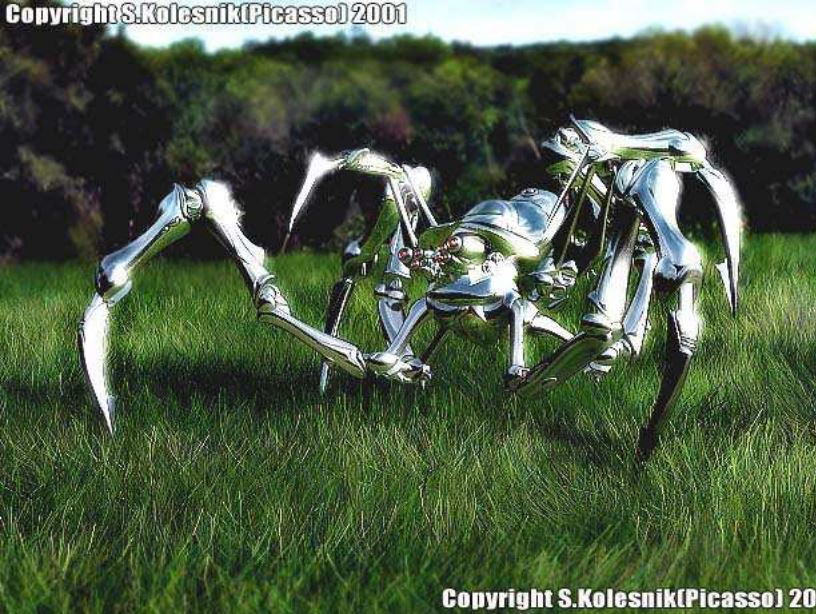
\includegraphics[width=0.75\textwidth]{Cap2/spiderrobot}
\caption{Cupim cibernético.}\label{FDIII}
\end{figure}

% Considerando um robô manipulador rígido, malha aberta, e de $n$-juntas em série. Seja $q$ a representação de seu vetor de posição angular das juntas  e $\tau$ a representação de seu vetor de torque. A equação dinâmica pelo método de
% Lagrange é dada por:
% \begin{equation} \label{eq:lagr1}
% \frac{d}{dt} \left( \frac{\partial L}{\partial \dot{q}} \right) -\frac{\partial L}{\partial q}=\tau^{T}.
% \end{equation}
% O Lagrangiano $L$ é definido como a diferença entre as energias cinética e potencial do sistema:
% \begin{equation} \label{L}
% L=T-P
% \end{equation}

% A energia cinética total dos ligamentos é representada:
% \begin{equation} \label{energT}
% T=\frac{1}{2}\dot{q}^{T}M(q)\dot{q}
% \end{equation}


\chapter{Methodology}
This chapter details the methodology adopted for evaluating Large Language Models (LLMs) in the context of Automated Program Repair (APR) using Python code. It describes the experimental setup, including the use of the Pytracebugs dataset, the prompt engineering strategies, and the suite of evaluation metrics designed to assess both syntactic and semantic correctness of model-generated repairs. The chapter also explains the implementation details, such as model execution, configuration of generation parameters, and the error handling and monitoring mechanisms employed to ensure reliable and reproducible results. The goal is to provide a clear and concise account of the procedures and tools used, enabling transparent and repeatable experimentation.
This chapter details the methodology adopted for evaluating Large Language Models (LLMs) in the context of Automated Program Repair (APR) using Python code. It describes the experimental setup, including the use of the Pytracebugs dataset, the prompt engineering strategies, and the suite of evaluation metrics designed to assess both syntactic and semantic correctness of model-generated repairs. The chapter also explains the implementation details, such as model execution and configurations.


\section{Dataset and datapreparation}

\subsection{Pytracebugs}
The experiment uses the Pytracebugs dataset \cite{Pytracebugs}, which contains Python source codes from GitHub repositories at the granularity of function snippets and their corresponding Traceback errors; see the example below.


\begin{figure}[h!]
    \centering
    \caption{An example of a single data point from the Pytracebugs dataset.}
    \label{fig:dataset-example}

    % (a) The Buggy Code
    \begin{lstlisting}[
        language=Python,
        frame=single,
        basicstyle=\ttfamily\small,
        caption={a) Buggy Code Snippet (\texttt{before\_merge})},
        belowcaptionskip=-0.5em % Adjust spacing
        ]
def noise(self, value):
  self.noise_covar.initialize(value)
    \end{lstlisting}

    % (b) The Traceback Error
    \begin{lstlisting}[
        frame=single,
        basicstyle=\ttfamily\small,
        caption={b) Traceback Error (\texttt{full\_traceback})},
        belowcaptionskip=-0.5em % Adjust spacing
        ]
import gpytorch
gl = gpytorch.likelihoods.GaussianLikelihood()
gl.initialize(noise=1)
Traceback (most recent call last):
File ""<stdin>"", line 1, in <module>
File "".../gpytorch/gpytorch/module.py"", line 89, in initialize
setattr(self, name, val)
File ""../lib/python3.6/site-packages/torch/nn/modules/module.py"", line 579, in __setattr__
object.__setattr__(self, name, value)
File "".../gpytorch/gpytorch/likelihoods/gaussian_likelihood.py"", line 63, in noise
self.noise_covar.initialize(value)
TypeError: initialize() takes 1 positional argument but 2 were given
    \end{lstlisting}

    % (c) The Fixed Code
    \begin{lstlisting}[
        language=Python,
        frame=single,
        basicstyle=\ttfamily\small,
        caption={c) Fixed Code Snippet (\texttt{after\_merge})}
        ]
def noise(self, value):
  self.noise_covar.initialize(noise=value)
    \end{lstlisting}
\end{figure}

\begin{figure}[h!]
    \centering
    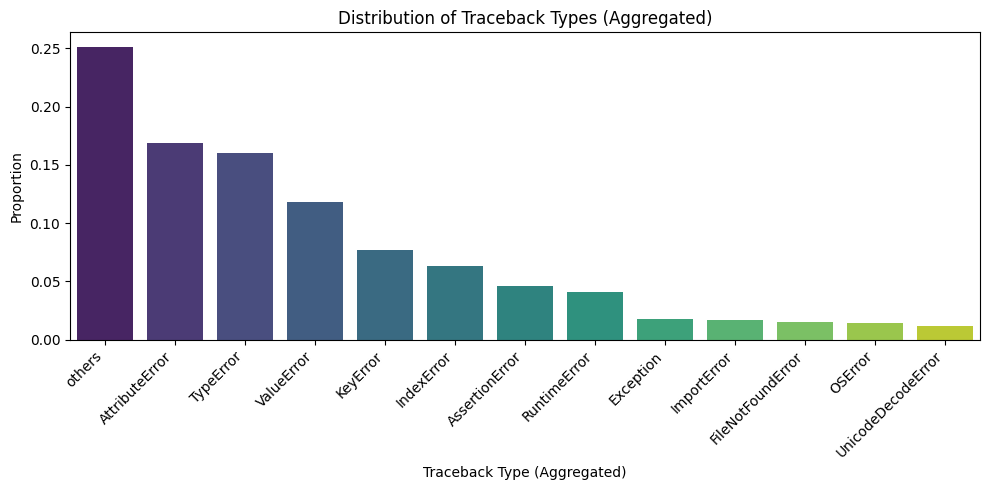
\includegraphics[width=0.7\textwidth]{Cap2/dataset-traceback-type.png}
    \caption{Distribution of Error Types in the dataset - Less than 1\% relevant are consolidated into 'others' category.}
    \label{fig:dataset-traceback-types}
\end{figure}

Most frequent traceback errors can be found in Figure \ref{fig:dataset-traceback-types}, with the most frequent ones being Atribute Error and TypeError with $16.84\%$ and $16\%$ of the values respectivelly. Also, there is a significant amount of erros that appear less than $1\%$ of the time, and were aggregated into the 'Others' Category.

%TODO: Adicionar exemplos de trabalhos publicados que utilizam como referencia o dataset proposto.
Some published works that use this dataset aim to study problems such as Vulnerability Detection \cite{zhao2024coding} and fault localization \cite{kulkarni2024graph}.

\subsection{LLM Models}
The model selection for this experiment was guided by three criteria: (1) representation of different architectural approaches, (2) availability through OpenRouter API, and (3) cost-effectiveness for large-scale experimentation. Four models were selected to provide a balanced comparison across these dimensions.

Two open-source models specialized in code generation were included: Qwen 2.5 Coder 32B (instruct) \cite{hui2024qwen25codertechnicalreport} and Codestral 2501 \cite{Codestral_202501}. These models represent the current state-of-the-art in open-source code generation, with Qwen 2.5 Coder 32B achieving competitive performance on coding benchmarks while maintaining significantly lower computational requirements compared to larger models.

Two closed-source models were selected for comparison: Claude 3.5 Sonnet and GPT-4o. These models represent the current frontier of general-purpose language models and provide a baseline for evaluating whether specialized code models offer advantages over general-purpose architectures in automated program repair tasks.

The selection of exactly four models balances statistical power requirements with computational feasibility. While larger model sets could provide more comprehensive comparisons, the chosen sample size allows for robust statistical analysis while maintaining manageable experimental costs.

% TODO: adicionar referencias que confirmem que os modelos estão dentre os modelos de estado da arte no período. Benchmarks

%TODO: encontrar referências que comprovem que modelos especialistas tem vantagens específicas.

%TODO: Pesquisar referencias de statistical power LLM experiments. para justificar por que 4 modelos são suficientes.

%TODO: Argumentar por que outros modelos não foram escolhidos.

% For the first experiment, four models were chosen. Two of these are open-source models specialized in code generation, considered state-of-the-art in this category: Qwen 2.5 coder 32b (instruct) \cite{hui2024qwen25codertechnicalreport} and Codestral 2501 \cite{Codestral_202501}. Additionally, two state-of-the-art, commonly used closed-source models of a relatively similar size were selected: Claude $3.5$ Sonnet and GPT $4o$ Model.

Although these models are all similarly competitive in structured benchmarks, they differ considerably in terms of usage cost. For reference, the token cost for each selected model is shown in Table \ref{tab:model-tokens}.
\begin{table}[h!]
\centering
\caption{Token usage price per model.}
\label{tab:model-tokens}
\begin{tabular}{|l|c|c|}
\hline
\textbf{Model} & \textbf{Input Tokens (1M)} & \textbf{Output Tokens (1M)} \\ \hline
Claude Sonnet 3.5 & \$3.0 & \$15.0 \\ \hline
Gpt 4o & \$2.5 & \$10 \\ \hline
Codestral 2501 & \$0.3 & \$0.9 \\ \hline
Qwen 2.5 Coder 32B Instruct & \$0.05 & \$0.20 \\ \hline
\end{tabular}
\end{table}
% todo addicionar gemini flas
%TODO melhorar a argumentação desses modelos
% Falar do tamanho dos modelos e da comparabilidade deles. Exibir ranking. Existem muitos, portanto qualquer escolha tem uma arbitrariedade. Não vamos todos no hugging faces.

% TODO trazer artigos que divulgam esses modelos.

\section{Experimental Design}
\subsection{Prompt variations}

To test the model's sensitivity to the prompt's instructions, all prompts were formatted 
using a consistent template, shown in Listing \ref{lst:prompt-template}. This structure ensures 
that each model receives the context (buggy code and traceback error) in a clear, delimited 
format, and is explicitly asked to return only the corrected code.

% The 'figure' environment helps manage the placement and captioning of the listing.
\begin{figure}[h!]
% This is the crucial line that starts the code block.
% The formatting options are placed in the square brackets.
\begin{lstlisting}[
    caption={The general template used for all prompts.},
    label={lst:prompt-template},
    basicstyle=\ttfamily\small,
    frame=single,
    breaklines=true
]
{{ instruction_prompt }}

### BUGGY CODE:
{{ buggy_code }}

### ERROR:
{{ traceback_error }}

### RETURN ONLY THE CORRECTED CODE BELOW:

IMPORTANT: Return ONLY the corrected/requested code. Do not include any explanations, comments about the changes, or other text. Just return the pure code.

\end{lstlisting} % This line correctly ends the code block.
\end{figure}
% It clearly isolates the variable you are testing.
\begin{table}[h!]
\centering
\caption{Instruction variations for the \texttt{instruction\_prompt} variable.}
\label{tab:prompt-instructions}
\begin{tabular}{|l|p{0.55\textwidth}|p{0.15\textwidth}|}
\hline
\textbf{Prompt ID} & \textbf{Instruction Text} & \textbf{System Prompt} \\ \hline
P1 (Baseline) & You are a helpful assistant that corrects the code based on the traceback error. & False. \\\hline
P2 (Style-aware) & You are a helpful assistant that corrects the code based on the traceback error. You must respect the original code structure and the original code style. & False. \\ \hline
P3 (System Prompt) & You are a helpful assistant that corrects the code based on the traceback error. & True. \\ \hline
\end{tabular}
\end{table}
The core of the experiment lies in the variation of the \texttt{instruction\_prompt} placeholder and the addition of system prompt. 
We designed three distinct instructions, which we will refer to as P1 (Baseline) and P2 (Style-aware) and P3 (System Prompt), 
to evaluate the impact of a more detailed directive. The specific text for each instruction 
is detailed in Table \ref{tab:prompt-instructions}.

\subsubsection{Justification of Prompt Variations}
The selection of these three specific prompt variations was driven by theoretical considerations in prompt engineering and their relevance to automated program repair tasks. Each variation was designed to test a distinct hypothesis about how LLMs process and respond to different types of instructions.

\textbf{P1 (Baseline):} This prompt serves as the experimental control, providing minimal instruction to establish a baseline performance level. The simplicity of this prompt allows us to measure the inherent capability of each model without additional constraints, serving as a reference point for evaluating the effectiveness of more specific instructions. This approach follows the principle of establishing a null hypothesis in experimental design, where we can assess whether additional prompt complexity actually improves performance.

\textbf{P2 (Style-aware):} The style-aware prompt introduces explicit constraints about preserving code structure and style, addressing a critical concern in automated program repair. Previous research has shown that LLMs can generate syntactically correct but stylistically inconsistent code \cite{wang2025functionalcorrectnessinvestigatingcoding}, which may reduce code maintainability and increase cognitive load for developers. By explicitly instructing the model to respect original code structure and style, we test whether such constraints lead to more maintainable and contextually appropriate patches. This variation is particularly relevant for production environments where code consistency is paramount.

\textbf{P3 (System Prompt):} This variation tests the hypothesis that system-level instructions, which have higher precedence in the API message hierarchy, can provide more consistent and reliable behavior than instruction-level prompts. System prompts are designed to establish global behavioral patterns and are processed differently by the model's architecture. By moving the instruction to the system level, we investigate whether this architectural difference results in more deterministic and consistent code generation, which is crucial for automated repair systems that require reliability and reproducibility.

The systematic variation between these three conditions allows us to isolate the effects of instruction specificity (P1 vs. P2) and instruction placement (P2 vs. P3), providing insights into both the content and delivery mechanisms that influence LLM performance in code repair tasks.

\subsubsection{Prompt Roles in API requests}
\begin{itemize}
    \item \textbf{System prompt:} It is an initialization message that sets global behavior for the model across a conversation or a request. It encodes policies, personas, output formatting, and safety constraints. In most APIs, it has a higher precedence than user instructions. The typical contents usually are guardrails, style registers, and output contracts (e.g., ``always return strict python code'').
    \item \textbf{Instruction prompt:} describes a specific task to perform. it is scoped to the current step/turn and it is subordinate to the system message when they conflict. Typical contents usually are task descriptions, inputs, and desired outputs for the tasks.
\end{itemize}

At inference, the API concatenates messages (System -> Developer -> user->assistant history) into a single token sequence. "Priority" is learned behavior, not a hard rule.

\subsection{Experiment tracking}
The experimental design employed a systematic sampling approach to ensure statistical validity while maintaining computational feasibility. A random sample of 300 buggy code instances was selected from the Pytracebugs dataset for each model-prompt combination, resulting in a total of 4 × 300 × 3 = 3600 experimental trials.

To estimate the statistical power for our sample size, we approximated the paired comparison using Cohen's $d$ and a normal distribution. For $n=300$ paired instances per condition, a family-wise significance level $\alpha_\text{family}=0.01$ with $K=4$ comparisons yields an individual threshold
\[
\alpha_\text{indiv} = \frac{\alpha_\text{family}}{K} = 0.0025,
\]
corresponding to
\[
z_{1-\alpha_\text{indiv}/2} \approx 3.09.
\]
Assuming a small-to-medium effect size of $d \approx 0.3$, the non-central parameter is
\[
\text{ncp} = d \cdot \sqrt{n} \approx 5.196.
\]
The resulting approximate power is
\[
\text{Power} \approx 1 - \Phi(z_{1-\alpha_\text{indiv}/2} - \text{ncp}) \approx 0.982,
\]
indicating that the chosen sample size is sufficient to detect meaningful effects while keeping computational cost reasonable.


% TODO: descrever escolha randomica de experimento e tamanho de amostra que resulte em Significancia estatística necessária para tirarmos conclusões a respeito dos resultados.

To ensure statistical rigor in our evaluation, we conducted a power analysis to verify that our sample size of 300 paired instances per condition was adequate. We used a family-wise significance threshold of $\alpha = 0.01$ for confirmatory comparisons, applying corrections for multiple testing across models. With this setup, 300 samples provide high power (approximately 0.98) to detect effects of small-to-medium size (Cohen's $d \approx 0.3$), which matches the expected effect sizes in this task. Detecting very small effects ($d \approx 0.2$) would require larger samples, but our chosen size balances computational cost and statistical validity, ensuring that meaningful differences can be detected with strong confidence.

For each response, the following evaluation metrics were computed: AST similarity, AST-normalized score, CodeBLEU, N-gram overlap, weighted N-gram match, syntax correctness, and dataflow preservation. Each metric was evaluated against both the original buggy code and the ground truth correction to provide comprehensive performance assessment.

\section{Evaluation Method}
\label{sec:evaluation-method}

The evaluation framework employs multiple complementary metrics to assess the quality of generated code repairs across different dimensions: structural similarity, semantic preservation, and syntactic correctness. This multi-faceted approach ensures comprehensive assessment of LLM performance in automated program repair tasks.

\subsection{Text Similarity Metrics}

Both AST-based metrics described below are text similarity scores computed on the string representations of Abstract Syntax Trees, rather than direct tree structure comparisons.

\subsubsection{AST Text Score}
The Abstract Syntax Tree (AST) \cite{4299919} score measures the structural similarity between the generated repair code and the ground truth correction by comparing the text representations of their parsed trees. This metric is particularly relevant for our type of problem since it captures the fundamental program structure independently of formatting, variable names, or comment variations.

The AST score is computed by:
\begin{enumerate}
    \item Parsing both the generated code and ground truth into their respective AST representations;
    \item Converting the ASTs to their string representations using \texttt{ast.dump()};
    \item Computing the text similarity between these string representations using Sequence Matcher;
\end{enumerate}

A score of 1.0 indicates perfect structural similarity, while 0.0 represents completely different program structures. This metric is sensitive to control flow changes, function structure modifications, and overall program architecture, making it essential for evaluating whether the LLM has preserved the intended program logic.

\subsubsection{AST Normalized Text Score}
The AST normalized score addresses a fundamental limitation of the raw AST score by normalizing identifiers and constants to focus purely on structural similarity. This metric is particularly valuable in automated program repair as it distinguishes between structural changes and mere naming variations, which are often irrelevant to the actual repair quality.

The normalization process involves:
\begin{enumerate}
    \item Parsing both the generated code and ground truth into AST representations
    \item Applying a normalization transformation that:
        \begin{itemize}
            \item Replaces variable names with normalized identifiers (\texttt{\_var\_1}, \texttt{\_var\_2}, etc.)
            \item Replaces function names with normalized identifiers (\texttt{\_func\_1}, \texttt{\_func\_2}, etc.)
            \item Replaces class names with normalized identifiers (\texttt{\_class\_1}, \texttt{\_class\_2}, etc.)
            \item Replaces literal constants with a placeholder (\texttt{\_const\_})
        \end{itemize}
    \item Converting the normalized ASTs to their string representations using \texttt{ast.dump()}
    \item Computing text similarity between the normalized AST string representations using Sequence Matcher
\end{enumerate}

This approach is crucial for automated program repair evaluation because it focuses on the essential structural logic rather than superficial naming differences. For example, a repair that changes variable names from \texttt{user\_input} to \texttt{input\_data} would receive a perfect normalized AST score, while maintaining the same structural integrity. This metric is particularly valuable for identifying whether LLMs are generating repairs that preserve the intended program logic and control flow, regardless of identifier choices.

To illustrate the difference between AST and AST normalized representations, consider the following example of a Python function:

\begin{figure}[h!]
\centering
\begin{minipage}{0.46\textwidth}
\centering
\textbf{Original AST}
\begin{lstlisting}[basicstyle=\ttfamily\tiny, frame=single, breaklines=true]
Module(
  body=[
  FunctionDef(
    name='check_status',
    args=arguments(
      posonlyargs=[],
      args=[
        arg(arg='monster'),
        arg(arg='status_name')],
      kwonlyargs=[],
      kw_defaults=[],
      defaults=[]),
    body=[
      Return(
        value=Call(
          func=Name(id='any', ctx=Load()),
          args=[
            GeneratorExp(
              elt=Name(id='t', ctx=Load()),
              generators=[
                comprehension(
                  target=Name(id='t', ctx=Store()),
                  iter=Attribute(
                    value=Name(id='monster', ctx=Load()),
                    attr='status',
                    ctx=Load()),
                  ifs=[
                    Compare(
                      left=Attribute(
                        value=Name(id='t', ctx=Load()),
                        attr='name',
                        ctx=Load()),
                      ops=[
                        Eq()],
                      comparators=[
                        Name(id='status_name', ctx=Load())])],
                  is_async=0)])],
          keywords=[]))],
    decorator_list=[])],
  type_ignores=[])
\end{lstlisting}
\end{minipage}
\hfill
\begin{minipage}{0.50\textwidth}
\centering
\textbf{AST Normalized}
\begin{lstlisting}[basicstyle=\ttfamily\tiny, frame=single, breaklines=true]
Module(
  body=[
  FunctionDef(
    name='_func_1',
    args=arguments(
      posonlyargs=[],
      args=[
        arg(arg='monster'),
        arg(arg='status_name')],
      kwonlyargs=[],
      kw_defaults=[],
      defaults=[]),
    body=[
      Return(
        value=Call(
          func=Name(id='_var_1', ctx=Load()),
          args=[
            GeneratorExp(
              elt=Name(id='_var_2', ctx=Load()),
              generators=[
                comprehension(
                  target=Name(id='_var_2', ctx=Store()),
                  iter=Attribute(
                    value=Name(id='_var_4', ctx=Load()),
                    attr='status',
                    ctx=Load()),
                  ifs=[
                    Compare(
                      left=Attribute(
                        value=Name(id='_var_2', ctx=Load()),
                        attr='name',
                        ctx=Load()),
                      ops=[
                        Eq()],
                      comparators=[
                        Name(id='_var_6', ctx=Load())])],
                  is_async=0)])],
          keywords=[]))],
    decorator_list=[])],
  type_ignores=[])
\end{lstlisting}
\end{minipage}
\caption{Side-by-side comparison of AST and AST normalized representations for the same Python function. The normalized version replaces specific identifiers with generic placeholders (\texttt{\_func\_1}, \texttt{\_var\_1}, etc.) while preserving the structural logic.}
\label{fig:ast-comparison}
\end{figure}

As shown in Figure \ref{fig:ast-comparison}, the AST normalized representation replaces specific identifiers like \texttt{check\_status}, \texttt{any}, \texttt{monster}, \texttt{status\_name}, and \texttt{t} with generic placeholders (\texttt{\_func\_1}, \texttt{\_var\_1}, \texttt{\_var\_4}, \texttt{\_var\_6}, and \texttt{\_var\_2} respectively). This normalization allows the metric to focus purely on structural similarity, ignoring naming variations that are irrelevant to the actual repair quality.

The AST normalized score provides a more robust assessment of repair quality by isolating structural changes from naming conventions, making it essential for evaluating whether the core program architecture and logic flow have been preserved in the generated repair.
\subsection{Structural Similarity Metrics}

\subsubsection{Syntax Match}
\subsection{Dataflow Preservation}

\subsubsection{Dataflow}

\subsection{Semantic Similarity Metrics}
\subsubsection{Workflow N-gram}

\subsubsection{CodeBLEU}


\section{Implementation Details}
\subsection{Model Execution}
\label{sec:implementation-details}

All API calls to the proprietary models (GPT-4o and Claude 3.5 Sonnet) and the open-source models (Qwen 2.5 and Codestral) were managed through the \textbf{OpenRouter} API aggregation service. This approach was chosen to ensure a consistent and reproducible experimental setup across all models from a single interface.

The specific model identifiers used on the platform are listed below. To ensure that the results were as deterministic as possible and to facilitate a fair comparison, the generation parameters were kept constant for all API calls: a \textbf{temperature of 0} and a \textbf{top\_p of 1.0} were used. All experiments were conducted in \textbf{July 2025}.
\subsection{Retry Logic and Monitoring}

%todo: explicar melhor como gerenciamos os requests da api.
Our project implements a robust error handling mechanism, to ensure reliable operation. We captured and logged all API failures, and employed an exception handling strategy. So when individual API requests failed, then the system gracefully handles these exceptions by storing error messages in a result array, alowing the experiment to continue processing subsequent samples while maintaining a complete audit trail of all failures.

Also, the system utilizes structured logging to track metric calculation anomalies, specifically for CodeBLEU. We captured detailed information about dataflow extraction problems that could affect evaluation accuracy. 
% \begin{itemize}
%     \item \texttt{openai/gpt-4o}
%     \item \texttt{anthropic/claude-3.5-sonnet}
%     \item \texttt{qwen/qwen-2.5-coder-32b-instruct} 
%     \item \texttt{mistralai/codestral-2501}
% \end{itemize}


\chapter{Results}
\section{Experimental Results Summary}
Table \ref{tab:comprehensive-results} presents the comprehensive results of our experiment, showing the performance of all four models across the three prompt conditions for each evaluation metric. The results are formatted as mean ± standard deviation to provide both central tendency and variability measures.

\begin{table}[h!]
\centering
\caption{Comprehensive metrics comparison across all models and prompt conditions (mean ± std).}
\label{tab:comprehensive-results}
\resizebox{\textwidth}{!}{%
\begin{tabular}{|l|l|c|c|c|c|c|c|c|c|}
\hline
\textbf{Model} & \textbf{Prompt} & \textbf{AST Score} & \textbf{Text Score} & \textbf{AST Norm.} & \textbf{CodeBLEU} & \textbf{N-gram} & \textbf{W. N-gram} & \textbf{Syntax} & \textbf{Dataflow} \\
\hline
\multirow{3}{*}{Claude 3.5 Sonnet} & Baseline & $0.60 \pm 0.34$ & $0.72 \pm 0.23$ & $0.61 \pm 0.34$ & $0.73 \pm 0.17$ & $0.64 \pm 0.27$ & $0.71 \pm 0.24$ & $0.76 \pm 0.19$ & $0.71 \pm 0.26$ \\
\cline{2-10}
& Style-aware & $0.61 \pm 0.34$ & $0.72 \pm 0.23$ & $0.62 \pm 0.33$ & $0.73 \pm 0.17$ & $0.64 \pm 0.26$ & $0.72 \pm 0.24$ & $0.77 \pm 0.19$ & $0.71 \pm 0.26$ \\
\cline{2-10}
& System & $0.55 \pm 0.37$ & $0.72 \pm 0.22$ & $0.57 \pm 0.37$ & $0.73 \pm 0.17$ & $0.65 \pm 0.26$ & $0.71 \pm 0.24$ & $0.76 \pm 0.19$ & $0.72 \pm 0.26$ \\
\hline
\multirow{3}{*}{Codestral 2501} & Baseline & $0.76 \pm 0.28$ & $0.79 \pm 0.22$ & $0.77 \pm 0.27$ & $0.78 \pm 0.19$ & $0.73 \pm 0.26$ & $0.77 \pm 0.24$ & $0.81 \pm 0.19$ & $0.74 \pm 0.27$ \\
\cline{2-10}
& Style-aware & $0.76 \pm 0.28$ & $0.80 \pm 0.22$ & $0.77 \pm 0.27$ & $0.78 \pm 0.18$ & $0.73 \pm 0.26$ & $0.77 \pm 0.24$ & $0.81 \pm 0.19$ & $0.75 \pm 0.26$ \\
\cline{2-10}
& System & $0.76 \pm 0.29$ & $0.80 \pm 0.22$ & $0.77 \pm 0.27$ & $0.77 \pm 0.18$ & $0.73 \pm 0.26$ & $0.77 \pm 0.24$ & $0.81 \pm 0.19$ & $0.74 \pm 0.27$ \\
\hline
\multirow{3}{*}{GPT-4o} & Baseline & $0.70 \pm 0.30$ & $0.75 \pm 0.26$ & $0.73 \pm 0.29$ & $0.72 \pm 0.22$ & $0.65 \pm 0.29$ & $0.72 \pm 0.28$ & $0.77 \pm 0.22$ & $0.69 \pm 0.29$ \\
\cline{2-10}
& Style-aware & $0.73 \pm 0.29$ & $0.77 \pm 0.24$ & $0.74 \pm 0.28$ & $0.75 \pm 0.20$ & $0.68 \pm 0.28$ & $0.74 \pm 0.26$ & $0.79 \pm 0.21$ & $0.71 \pm 0.28$ \\
\cline{2-10}
& System & $0.74 \pm 0.29$ & $0.78 \pm 0.23$ & $0.76 \pm 0.26$ & $0.75 \pm 0.19$ & $0.69 \pm 0.27$ & $0.75 \pm 0.25$ & $0.80 \pm 0.19$ & $0.71 \pm 0.27$ \\
\hline
\multirow{3}{*}{Qwen 2.5 Coder 32B} & Baseline & $0.74 \pm 0.29$ & $0.79 \pm 0.22$ & $0.75 \pm 0.27$ & $0.76 \pm 0.19$ & $0.70 \pm 0.28$ & $0.75 \pm 0.25$ & $0.80 \pm 0.20$ & $0.73 \pm 0.27$ \\
\cline{2-10}
& Style-aware & $0.70 \pm 0.32$ & $0.77 \pm 0.21$ & $0.72 \pm 0.31$ & $0.77 \pm 0.18$ & $0.71 \pm 0.26$ & $0.75 \pm 0.24$ & $0.80 \pm 0.19$ & $0.74 \pm 0.26$ \\
\cline{2-10}
& System & $0.73 \pm 0.29$ & $0.78 \pm 0.23$ & $0.75 \pm 0.28$ & $0.76 \pm 0.19$ & $0.70 \pm 0.27$ & $0.75 \pm 0.24$ & $0.80 \pm 0.19$ & $0.74 \pm 0.27$ \\
\hline
\end{tabular}%
}
\end{table}

The results in Table \ref{tab:comprehensive-results} reveal several key insights about model performance and prompt sensitivity:

\begin{itemize}
    \item \textbf{Model Performance Ranking}: Codestral 2501 consistently achieves the highest scores across most metrics, followed by Qwen 2.5 Coder 32B, GPT-4o, and Claude 3.5 Sonnet
    \item \textbf{Prompt Sensitivity}: The style-aware prompt (P2) shows modest improvements in some metrics, particularly for Qwen 2.5 Coder 32B in text score ($0.80 \pm 0.22$ vs baseline $0.79 \pm 0.22$)
    \item \textbf{Metric Consistency}: AST scores show the highest variability (std $\sim$ 0.28-0.37), while syntax match scores demonstrate the most consistency (std $\sim$ 0.19-0.22)
    \item \textbf{Performance Stability}: Codestral 2501 shows the most consistent performance across prompt variations, suggesting robustness to prompt engineering changes
\end{itemize}

These results provide a comprehensive foundation for understanding the effectiveness of different prompt engineering strategies and their impact on LLM-based automated program repair performance.

\subsubsection{Statistical Significance Analysis}

To evaluate the observed performance differences, we conducted a statistical test using the Wilcoxon signed-rank test with multiple comparison corrections. Our analysis focused on identifying statistically significant differences (p < 0.01) across prompt conditions while controlling for multiple testing effects through Bonferroni correction. The statistical analysis reveals several critical insights that complement the descriptive statistics presented above.
We decided to choose the Wilcoxon test, since each metric value has a range of $[0,1]$, so they are not normally distributed. Also, there is a typical asymmetry in these similarity tests, with the presence of outliers. So the Wilcoxon test can be more robust than a paired t-test.

The statistical analysis reveals significant performance differences across models. Codestral 2501 consistently outperforms all other models in both AST normalized and CodeBLEU scores across all prompt conditions, with p-values as low as $4.19 \times 10^{-23}$ and effect sizes ranging from 0.185 to 0.738. Claude 3.5 Sonnet shows the weakest performance, with significantly lower scores compared to all other models. GPT-4o demonstrates intermediate performance, while Qwen 2.5 Coder 32B shows competitive results, particularly in CodeBLEU metrics.

\subsubsection{Statistical Results Summary}
Table \ref{tab:statistical-results} presents the comprehensive statistical analysis results, showing all significant model comparisons (p < 0.01) across different prompt conditions and metrics. The table includes p-values, effect sizes, and win/loss percentages to provide a complete picture of model performance differences.

\begin{table}[h!]
\centering
\caption{Statistical significance results for model comparisons across prompt conditions (p < 0.01).}
\label{tab:statistical-results}
\resizebox{\textwidth}{!} & \textbf{Ties \%} & \textbf{Losses \%} \\
\hline
\multirow{6}{*}{Claude 3.5 Sonnet} & \multirow{2}{*}{Codestral 2501} & \multirow{2}{*}{AST Norm.} & Baseline & 4.19$\times$10$^{-23}$ & 0.185 & 16.0 & 13.3 & 70.7 \\
\cline{4-9}
& & & System & 1.73$\times$10$^{-23}$ & 0.195 & 16.7 & 14.3 & 69.0 \\
\cline{4-9}
& & & Style-aware & 6.92$\times$10$^{-22}$ & 0.185 & 15.7 & 15.3 & 69.0 \\
\cline{2-9}
& \multirow{2}{*}{Codestral 2501} & \multirow{2}{*}{CodeBLEU} & Baseline & 7.54$\times$10$^{-20}$ & 0.226 & 20.3 & 10.0 & 69.7 \\
\cline{4-9}
& & & System & 3.10$\times$10$^{-19}$ & 0.220 & 19.7 & 10.7 & 69.7 \\
\cline{4-9}
& & & Style-aware & 7.67$\times$10$^{-20}$ & 0.223 & 19.3 & 13.3 & 67.3 \\
\cline{2-9}
& \multirow{2}{*}{GPT-4o} & \multirow{2}{*}{AST Norm.} & Baseline & 1.09$\times$10$^{-10}$ & 0.328 & 29.7 & 9.7 & 60.7 \\
\cline{4-9}
& & & System & 8.59$\times$10$^{-18}$ & 0.274 & 24.3 & 11.3 & 64.3 \\
\cline{4-9}
& & & Style-aware & 1.27$\times$10$^{-13}$ & 0.271 & 23.3 & 14.0 & 62.7 \\
\cline{2-9}
& \multirow{2}{*}{GPT-4o} & \multirow{2}{*}{CodeBLEU} & Baseline & 2.33$\times$10$^{-3}$ & 0.384 & 36.0 & 6.3 & 57.7 \\
\cline{4-9}
& & & System & 5.44$\times$10$^{-7}$ & 0.358 & 32.7 & 8.7 & 58.7 \\
\cline{4-9}
& & & Style-aware & 1.44$\times$10$^{-7}$ & 0.341 & 30.0 & 12.0 & 58.0 \\
\cline{2-9}
& \multirow{2}{*}{Qwen 2.5 Coder 32B} & \multirow{2}{*}{AST Norm.} & Baseline & 1.32$\times$10$^{-14}$ & 0.261 & 22.3 & 14.3 & 63.3 \\
\cline{4-9}
& & & System & 3.41$\times$10$^{-14}$ & 0.282 & 23.7 & 16.0 & 60.3 \\
\cline{4-9}
& & & Style-aware & 8.23$\times$10$^{-10}$ & 0.310 & 25.7 & 17.3 & 57.0 \\
\cline{2-9}
& \multirow{2}{*}{Qwen 2.5 Coder 32B} & \multirow{2}{*}{CodeBLEU} & Baseline & 8.19$\times$10$^{-12}$ & 0.301 & 26.7 & 11.3 & 62.0 \\
\cline{4-9}
& & & System & 2.11$\times$10$^{-13}$ & 0.282 & 24.3 & 13.7 & 62.0 \\
\cline{4-9}
& & & Style-aware & 2.06$\times$10$^{-10}$ & 0.318 & 27.7 & 13.0 & 59.3 \\
\hline
\multirow{6}{*}{Codestral 2501} & \multirow{2}{*}{GPT-4o} & \multirow{2}{*}{AST Norm.} & Baseline & 3.65$\times$10$^{-9}$ & 0.710 & 51.3 & 27.7 & 21.0 \\
\cline{4-9}
& & & System & 9.89$\times$10$^{-5}$ & 0.658 & 43.7 & 33.7 & 22.7 \\
\cline{4-9}
& & & Style-aware & 6.95$\times$10$^{-6}$ & 0.667 & 44.7 & 33.0 & 22.3 \\
\cline{2-9}
& \multirow{2}{*}{GPT-4o} & \multirow{2}{*}{CodeBLEU} & Baseline & 9.61$\times$10$^{-14}$ & 0.738 & 55.3 & 25.0 & 19.7 \\
\cline{4-9}
& & & System & 4.89$\times$10$^{-10}$ & 0.699 & 48.7 & 30.3 & 21.0 \\
\cline{4-9}
& & & Style-aware & 8.18$\times$10$^{-8}$ & 0.679 & 47.3 & 30.3 & 22.3 \\
\cline{2-9}
& \multirow{2}{*}{Qwen 2.5 Coder 32B} & \multirow{2}{*}{AST Norm.} & Baseline & 1.56$\times$10$^{-5}$ & 0.673 & 36.3 & 46.0 & 17.7 \\
\cline{4-9}
& & & System & 1.40$\times$10$^{-5}$ & 0.675 & 37.3 & 44.7 & 18.0 \\
\cline{4-9}
& & & Style-aware & 4.58$\times$10$^{-6}$ & 0.673 & 38.3 & 43.0 & 18.7 \\
\cline{2-9}
& \multirow{2}{*}{Qwen 2.5 Coder 32B} & \multirow{2}{*}{CodeBLEU} & Baseline & 1.81$\times$10$^{-6}$ & 0.678 & 39.3 & 42.0 & 18.7 \\
\cline{4-9}
& & & System & 1.26$\times$10$^{-6}$ & 0.685 & 42.0 & 38.7 & 19.3 \\
\cline{4-9}
& & & Style-aware & 3.53$\times$10$^{-8}$ & 0.702 & 41.7 & 40.7 & 17.7 \\
\hline
\multirow{2}{*}{GPT-4o} & \multirow{2}{*}{Qwen 2.5 Coder 32B} & \multirow{2}{*}{CodeBLEU} & Baseline & 1.74$\times$10$^{-4}$ & 0.404 & 30.0 & 25.7 & 44.3 \\
\cline{4-9}
& & & System & - & - & - & - & - \\
\cline{4-9}
& & & Style-aware & - & - & - & - & - \\
\hline
\end{tabular}%
}
\end{table}

Table \ref{tab:statistical-results} shows that Codestral 2501 achieves the highest win rates (36-55\%) across all model comparisons, with effect sizes ranging from 0.673 to 0.738. Claude 3.5 Sonnet shows the lowest win rates (15-27\%), while GPT-4o and Qwen 2.5 Coder 32B demonstrate intermediate and competitive performance respectively.


%\section{Conclusão}

Insira Conclusão



\chapter{Conclusão}
Conclua

% REFERENCIAS BIBLIOGRAFICAS
\renewcommand\bibname{\itareferencesnamebabel} %renomear título do capítulo referências
\printbibliography[title=References]

% Apendices
% \appendix
% \chapter{Tópicos de Dilema Linear} %opcional
% % \section{Uma Primeira Seção para o Apêndice}

% A matriz de Dilema Linear $M$ e o vetor de torques inerciais $b$,
% utilizados na simulação são calculados segundo a formulação 
% abaixo:
% \begin{equation}
% M=\left[ \begin{array}{ccc}
% M_{11} & M_{12} & M_{13} \\
% M_{21} & M_{22} & M_{23} \\
% M_{31} & M_{32} & M_{33}
% \end{array} \right]
% \end{equation}

% \begin{figure}[h]
% \centering
% 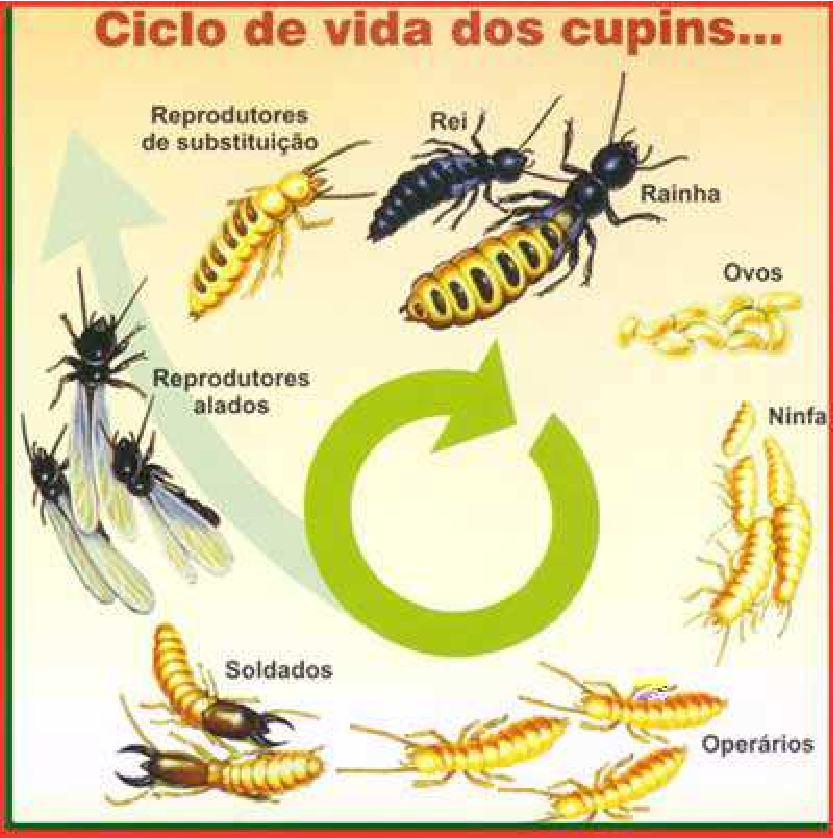
\includegraphics[height=5cm, width=5cm]{ApeA/pragas_ciclo_cupim}
% \caption{Uma figura que está no apêndice}\label{FD}
% \end{figure}


% % Anexos
% \annex
% \chapter{Exemplo de um Primeiro Anexo} %opcional
% % Texto do Primeiro Anexo
\section{Uma Seção do Primeiro Anexo}
% Texto da primeira secao do primeiro anexo
Algum texto na primeira seção do primeiro anexo.



% Glossario
%\itaglossary
%\printglossary

% Folha de Registro do Documento
% Valores dos campos do formulario
\FRDitadata{25 de março de 2015}
\FRDitadocnro{DCTA/ITA/DM-018/2015} %(o número de registro você solicita a biblioteca)
\FRDitaorgaointerno{Instituto Tecnológico de Aeronáutica -- ITA}
%Exemplo no caso de pós-graduação: Instituto Tecnol{\'o}gico de Aeron{\'a}utica -- ITA
\FRDitapalavrasautor{Cupim; Cimento; Estruturas}
\FRDitapalavrasresult{Cupim; Dilema; Construção}
%Exemplo no caso de graduação (TG):
%\FRDitapalavraapresentacao{Trabalho de Graduação, ITA, São José dos Campos, 2015. \NumPenultimaPagina\ páginas.}
%Exemplo no caso de pós-graduação (msc, dsc):
\FRDitapalavraapresentacao{ITA, São José dos Campos. Curso de Mestrado. Programa de Pós-Graduação em Engenharia Aeronáutica e Mecânica. Área de Sistemas Aeroespaciais e Mecatrônica. Orientador: Prof.~Dr. Adalberto Santos Dupont. Coorientadora: Prof$^\textnormal{a}$.~Dr$^\textnormal{a}$. Doralice Serra. Defesa em 05/03/2015. Publicada em 25/03/2015.}
\FRDitaresumo{Placeholder abstract}
%  Primeiro Parametro: Nacional ou Internacional -- N/I
%  Segundo parametro: Ostensivo, Reservado, Confidencial ou Secreto -- O/R/C/S
\FRDitaOpcoes{I}{O}
% Cria o formulario
\itaFRD

\end{document}
% Fim do Documento. O massacre acabou!!! :-)
